\documentclass[11pt,a4paper, twocolumn]{article}
\usepackage[utf8x]{inputenc}
\usepackage[czech]{babel}
\usepackage[IL2]{fontenc}
\usepackage[left=1.5cm,right=1.5cm,top=2.5cm,bottom=2cm]{geometry}
\usepackage{amsmath}
\usepackage{amsfonts}
\usepackage{amssymb}
\usepackage{amsthm}

\usepackage[]{xspace}
\usepackage[]{verbatim}
\usepackage{times}
\providecommand{\uv}[1]{\quotedblbase #1\textquotedblleft}
\newcommand{\latex}{\LaTeX\xspace}

\theoremstyle{definition}
\newtheorem{defn}{Definice}[section]

\theoremstyle{plain}	
\newtheorem{algr}[defn]{Algoritmus}
\newtheorem{veta}{Věta}

\author{Viktor Jančík}
\begin{document}
\begin{titlepage}

% \vspace*{1cm}
\begin{figure}[!h]
  \centering
  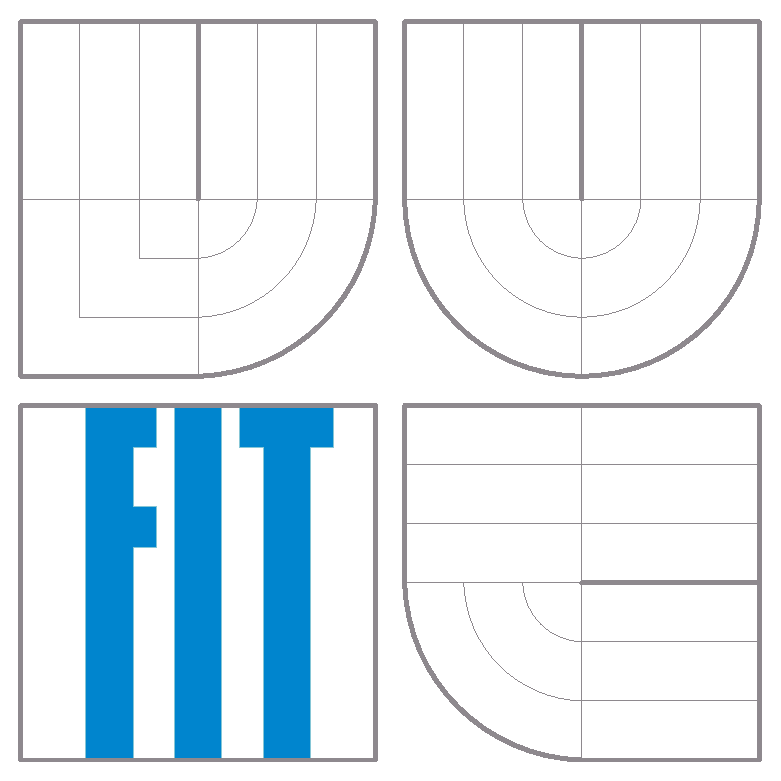
\includegraphics[height=5cm]{img/logo}
\end{figure}

\vfill

\begin{center}
\begin{Large}
Téoria obvodov\\
\end{Large}
\bigskip
\begin{Huge}
Semestrálny projekt\\
\end{Huge}
\end{center}

\vfill

\begin{center}
\begin{Large}
\today
\end{Large}
\end{center}

\vfill

\begin{flushleft}
\begin{large}
\begin{tabular}{ll}
Autor: 
 & Viktor Jančík, \url{xjanci09@stud.fit.vutbr.cz} \\
 & Fakulta Informačních Technologií \\
 & Vysoké Učení Technické v~Brně \\
\end{tabular}
\end{large}
\end{flushleft}
\end{titlepage}


\section*{Úvod}

V této úloze si vyzkoušíme sazbu titulní strany, matematických vzorců, prostředí a dalších textových struktur obvyklých pro technicky zaměřené texty (například rovnice (\ref{eq:first}) nebo definice \ref{def:oneone} na straně \pageref{def:oneone}).

Na titulní straně je využito sázení nadpisu podle optického středu s využitím zlatého řezu. Tento postup byl probírán na přednášce.

\section{Matematický text}

Nejprve se podíváme na sázení matematických symbolů a~výrazů v plynulém textu. Pro množinu $V$ označuje card($V$) kardinalitu $V$.
Pro množinu $V$ reprezentuje $V^*$ volný monoid generovaný množinou $V$ s operací konkatenace.
Prvek identity ve volném monoidu $V^*$ značíme symbolem $\varepsilon$
Nechť $V^+ = V^* - \{\varepsilon\}$ Algebraicky je tedy $V^+$ volná pologrupa generovaná množinou $V$ s operací konkatenace.
Konečnou neprázdnou množinu $V$ nazvěme abeceda.
Pro $w \in V^*$ označuje $|w|$ délku řetězce $w$. Pro $W \subseteq V$ označuje occur($w,W$) počet výskytů symbolů z $W$ v řetězci $w$ a sym($w,i$) určuje $i$-tý symbol řetězce $w;$ například sym($abcd,3) = c$.

Nyní zkusíme sazbu definic a vět s využitím balíku \verb|amsthm|.

\begin{defn}\label{def:oneone}Bezkontextová gramatika je čtveřice $G=(V,T,P,S)$, kde $V$ je totální abeceda,
$T \subseteq V$ je abeceda terminálů, $S\in(V-T)$ je startující symbol a $P$ je konečná množina pravidel
tvaru $q: A \rightarrow \alpha$, kde $A\in (V-T)$, $a\in V^*$ a $q$ je návěští tohoto pravidla. Nechť $N = V-T$ značí abecedu neterminálů.
Pokud $q: A \rightarrow \alpha \in P, \gamma, \delta \in V^*, G$ provádí derivační krok z $\gamma A \delta$ do $\gamma \alpha \delta$ podle pravidla $q: A \rightarrow \alpha$, symbolicky píšeme 
$\gamma A \delta \Rightarrow \gamma \alpha \delta$ $[q: A \rightarrow \alpha ]$ nebo zjednodušeně $\gamma A \delta \Rightarrow \gamma \alpha \delta$. Standardním způsobem definujeme $\Rightarrow ^m$, kde $m\geq 0$. Dále definujeme 
tranzitivní uzávěr $\Rightarrow ^+$ a tranzitivně-reflexivní uzávěr $\Rightarrow ^*$. \end{defn}

Algoritmus můžeme uvádět podobně jako definice textově, nebo využít pseudokódu vysázeného ve vhodném prostředí (například \verb|algorithm2e|).


\begin{algr}Algoritmus pro ověření bezkontextovosti gramatiky. Mějme gramatiku $G = (N, T, P, S)$.
\begin{enumerate}
 \item Pro každé pravidlo $p\in P$ proveď test, zda $p$ na levé straně obsahuje právě jeden symbol z $N$.
 \item Pokud všechna pravidla splňují podmínku z kroku $1$, tak je gramatika $G$ bezkontextová.
\end{enumerate} 
\end{algr}

\begin{defn}Jazyk definovaný gramatikou $G$ definujeme jako $L(G) = \{ w\in T^*|S \Rightarrow ^* w\}$ .\end{defn}

\subsection{Podsekce obsahující větu}

\begin{defn}Nechť $L$ je libovolný jazyk. $L$ je $\text{\textit{bezkontextový jazyk}}$, když a jen když $L=L(G)$, kde $G$ je libovolná bezkontextová gramatika.\end{defn}

\begin{defn}Množinu $\mathcal{L}_{CF} = \{L|L$ je bezkontextový jazyk$\}$ nazýváme $\text{\textit{třídou bezkontextových jazyků.}}$\end{defn}

\begin{veta}\label{thm:first} Nechť $L_{abc} = \{ a^nb^nc^n|n \geq 0\}$ Platí, že $L_{abc} \not\in \mathcal{L}_{CF}$\end{veta}

\begin{proof}[Důkaz] Důkaz se provede pomocí Pumping lemma pro bezkontextové jazyky, kdy ukážeme, že není možné, aby platilo, což bude implikovat pravdivost věty \ref{thm:first}.
\end{proof}

\section{Rovnice a odkazy}

Složitější matematické formulace sázíme mimo plynulý text. Lze umístit několik výrazů na jeden řádek, ale pak je třeba tyto vhodně oddělit, například příkazem \verb|\quad|.

\[ \sqrt[x^2]{y_0^3} \quad \mathbb{N} = \{ 0,1,2, \ldots \} \quad x^{y^y} \neq x^{yy} \quad z_{i_j} \not \equiv z_{ij} \]

V rovnici (\ref{eq:first}) jsou využity tři typy závorek s různou explicitně definovanou velikostí.

\begin{equation}\label{eq:first}
\bigg\{ \Big[ \big( a+b \big) * c \Big] ^d + 1 \bigg\} = x
\end{equation}

\[ \lim_{x\to\infty} \frac{sin^2x+cos^2x}{4}=y \]

V této větě vidíme, jak vypadá implicitní vysázení limity $\lim_{n\to\infty} f(n)$ v normálním odstavci textu. Podobně je to i s dalšími symboly jako $\sum_1^n$ či $\bigcup_{A\in B}$ . V případě vzorce $\lim\limits_{x\to\infty}\frac{\sin x}{x} = 1$ jsme si vynutili méně úspornou sazbu příkazem \verb|\limits|.

\begin{align}
\int\displaylimits_a^b f(x)dx &= - \int_b^a f(x)dx \\
\Big( \sqrt[5]{x^4} \Big)^\prime = \Big( x^{\frac{4}{5}} \Big)^\prime &= \frac{4}{5}x^{-\frac{1}{5}} = \frac{4}{5 \sqrt[5]{x}} \\
\overline{\overline{A \vee B}} &= \overline{\overline{A} \wedge \overline{B}}
\end{align}

\section{Matice}

Pro sázení matic se velmi často používá prostředí \verb|array| a závorky (\verb|\left,\right|). 

\[\left(
\begin{array}{c c c}
  a+b & b-a \\
  \widehat{e+w} & \hat{\pi} \\
  \vec{a}  & \stackrel{\longleftrightarrow}{AC}  \\
  0 & \beta
\end{array}
\right)\] 	

\[ \mathbf{A} =
\left\|
\begin{array}{c c c c c}
  a_{11} & a_{12} & \cdots & a_{1n} \\
  a_{21} & a_{22} & \cdots & a_{2n} \\
  \vdots  & \vdots  & \ddots & \vdots  \\
  a_{m1} & a_{m2} & \cdots & a_{mn}
\end{array}
\right\| \]

\[ \left|
\begin{array}{c c}
  t & u \\
  v & w
\end{array}
\right|
= tw - uv \]

Prostředí \verb|array| lze úspěšně využít i jinde.

\[ {n \choose k} = \left\{ 
  \begin{array}{c l}
    {n! \over k!(n-k)!} & \text{pro $0 \leq k \leq n$}\\
    0 & \text{pro $k < 0$ nebo $k > n$}
  \end{array} \right.
\]

\section{Závěrem}

V případě, že budete potřebovat vyjádřit matematickou konstrukci nebo symbol a nebude se Vám dařit jej nalézt v samotném {\LaTeX}u, doporučuji prostudovat možnosti balíku maker \AmS-\LaTeX.
Analogická poučka platí obecně pro jakoukoli konstrukci v {\TeX}u.

\end{document}